\chapter{Háttérismeretek}

A célja ennek a fejezetnek, hogy átadjam a témám értelmezéséhez szükséges alapismereteket, fogalmakat és bemutassam a használt technikai eszközöket. Ebben a fejezetben leírtak lesznek szükségesek ahhoz, hogy a későbbi fejezeteket teljességükben lehessen értelmezni.

Először szeretném a későbbiekben használt szakszavakat definiálni, az elterjedt szakirodalmakban található leírások alapján. 

Majd ezután írok az autóipari kiberbiztonság szabályozási környezetéről, azon belül is elsősorban az ISO/SAE 21434 szabványról fogok írni, ami lefedi alapvető irányelveket ehhez a területhez, valamint ad egy kezdetleges metodológiát a kiberbiztonsági kockázatelemzésre.

Később adok egy leírást az IT biztonság területén már ismert fenyegetésmodellezés technikákról és keretrendszerekről.

Végül pedig adok egy rövid leírást a munkám során alkalmazott eszközökről és technológiákról.

\section{Kiberbiztonsághoz kapcsolódó alapfogalmak}

Ebben a fejezetben található minden továbbiakban nem általánosnak vehető, az autóipari és a kiberbiztonsági területeken használt szakszavaknak a definíciói. Ezek a leírások elsősorban a már elérhető kutatásoknak, szabályozásoknak és szabványoknak a szójegyzékére építenek.

\begin{itemize}
    \item \textbf{Termék (product / item):} Egy önmagában is értelmezhető és értékesíthető rendszer, amelynek a biztonságát biztosítani kell. Ez lehet egy komponens vagy komponensek csoportja és egy jármű-szintű funkcionalitást valósít meg, pl. kormányrendszer, fékrendszer, szoftver-frissítési infrastruktúra
    \item \textbf{Komponens (component):} Logikailag és/vagy technikailag szeparálható elem    
    \item \textbf{Úthasználó (road user):} Személy aki valamilyen formában az utat használja, pl. gyalogos, autóvezető, utas, stb.
    \item \textbf{Kiberbiztonsági terv (cybersecurity concept):} Kiberbiztonsági követelményei egy terméknek, az üzemeltetési környezetnek, támogató információk a mitigációkhoz
    \item \textbf{Kiberbiztonsági specifikáció (cybersecurity specification):} Részletesebb kiberbiztonsági követelmények allokálva az architektúrális tervre
    \item \textbf{Kiberbiztonsági cél (cybersecurity goal):} Magas-szintű kiberbiztonsági követelmény
    \item \textbf{Kiberbiztonsági állítás (cybersecurity claim):} Állítás egy kockázatról
    \item \textbf{Mitigáció (mitigation / cybersecurity control):} Kockázatmódosító intézkedés
    \item \textbf{Érték (asset):} Egy tárgy ami értékkel rendelkezik
    \item \textbf{Kiberbiztonsági tulajdonság (cybersecurity property):} Egy attribútum amelyet meg kell védeni, pl. sértetlenség, bizalmasság, elérhetőség
    \item \textbf{Károkozás (damage scenario):} Egy kedvezőtlen következmény amely hatással van az úthasználóra
    \item \textbf{Fenyegetés (threat scenario):} Egy lehetséges kompromittálása valamilyen érték kiberbiztonsági tulajdonságának, amely egy károkozáshoz vezethet (pl: egy szoftveres sérülékenység kihasználása)
    \item \textbf{Támadási útvonal (attack path):} Események (pl: egy fenyegetés megvalósulása) egymás utáni bekövetkezése, amelyek egy fenyegetést realizál
    \item \textbf{Támadási lépés (attack step):} Az egyes események amelyeknek az egymás utáni sorozata egy támadási útvonalat realizál
\end{itemize}

\section{Autóipari kiberbiztonsági szabályozások és szabványok}

Az autóipari kiberbiztonság területe ellentétben az üzembiztonsággal vagy a bővebb IT biztonsággal még csak pár éves múltra tekint vissza, emiatt az itt alkalmazandó szabályozások és szabványok még csak az első alkalommal kerültek kiadásra. 

\subsection{UN ECE R155}
Az első specifikusan autóipari szabályozás az Egyesült Nemzetek által kiadott 155-ös számú szabályozás a kiberbiztonságról és a kiberbiztonság kezelő rendszerekről és járművek engedélyeztetésének kapcsolatáról (UN ECE R155\cite{R155}). Ennek a szabályozásnak kell megfelelnie a járműgyártóknak és beszállítóiknak az összes 2024 után megjelenő járműmodell engedélyeztetéséhez.

Ez a szabályozás már tartalmazza az igényt a kockázat-alapú kiberbiztonsági kezelés szükségességére. Ami annyit tesz, hogy a biztonsági szolgáltatásokat az alapján kell meghatározni, hogy egy kiberbiztonsági fenyegetés esetleges bekövetkezése mekkora hatással lenne a védendő autóipari termékre.

Szintén már megtalálhatjuk az autóipari termékek életciklusának különválasztását fejlesztési, gyártási és gyártás utáni fázisokra, ami mutatja azt, hogy a kiberbiztonsági szempontból fontos figyelembe, venni, hogy az életciklus különböző szakaszain más-más fenyegetésekre lehet számítani, valamint ez alapján más követelmények is lesznek érvényesek a termékre.

A dokumentum a továbbiakban követelményeket határoz meg, hogy milyen folyamatokon kell keresztülmennie egy autóipari terméknek, ahhoz, hogy az a közúti használatra engedélyt kapjon. 

\subsection{ISO/SAE 21434}

A másik, már technikaibb szintű, szintén 2021-es megjelenésű, irányadó szabvány az autóipari kiberbiztonsági mérnökségről szóló ISO/SAE 21434 "Road vehicles - Cybersecurity engineering". Ezt a szabványt közösen fejlesztette és adta ki 2021 augusztusában az International Standards Organization (ISO) és a Society of Automotive Engineers (SAE).

Ez a szabvány kezdett el követelményeket megfogalmazni az autóipari rendszerek (E/E) kiberbiztonsági kockázatkezelésének menetére, valamint a biztonság fejlesztésére és kezelésére. A felépítése emlékezetheti az olvasóját a már jóval ismertebb ISO 26262 "Road vehicles - Functional safety" szabványra, amely ugyanazon termékeknek az üzembiztonság kezelésére és elemzésére fókuszál.

Kezdésképpen a szabvány tervezési, fejlesztési, gyártási, üzemeltetési, karbantartási és kivezetési fázisaira fogalmaz meg követelményeket, valamint tartalmaz egy fenyegetés elemző és kockázat értékelő eljárást amelynek a Threat Analysis and Risk Assessment (TARA) nevet adták.

Továbbá tartalmaz más követelményeket a kiberbiztonsági elvárások kezelésére menedzsment és organizációs szintekre, azonban ezek ismerete nem tartozik a témám látókörébe.

Maga a téma kifejezetten a tervezési fázishoz tartozó kockázatelemzésnek a végrehajtására vonatkozó követelményeit veszi alapul. A később bemutatásuk során felfedezhető lesz, hogy nem elhanyagolható szüksége van a kockázatelemzés iteratív használatának eltérően az életciklus fázisaira, azonban a termék üzemeltetési környezetére vonatkozó védelmet ebben a fázisban határozzuk meg.

\subsubsection{Követelmények a tervezési fázisra}
A tervezési fázis egy autóipari termék életciklusában a kiindulópont. Az ebben a fázisban végzett kiberbiztonsági tevékenységek célja, hogy (i) definiálásra kerüljön az elemzendő termék, a környezete és interakciói, (ii) meghatározzák a kiberbiztonsági célokat és állításokat valamint, hogy (iii) elkészüljön a kiberbiztonsági terv.

A \textbf{termék definíciója} tartalmazza a termék határait, feladatait, valamint az előzetes architektúrát. Célunk itt az, hogy összegyűjtsük az elemzéshez szükséges információkat.

A \textbf{kiberbiztonsági célok és állítások} meghatározásához szükséges a TARA elvégzése, amelynek a kimenete, az egyes kockázatok kezelésére vonatkozó döntések lesznek, amelyek alapján eldönthetjük, hogy a kockázathoz egy célt vagy állítást kell megfogalmaznunk. A cél fogja meghatározni a magas-szintű követelményt amit a termék fejlesztése során figyelembe kell venni, míg az állítás azt határozza meg, hogy az adott kockázat mitigálása valamilyen okból már teljesül vagy a teljesülése szükségtelen.

Ezután készülhet el a \textbf{kiberbiztonsági terv}, amelyben az egyes mitigációkat határozzuk meg a célok elérésére, a célokat tovább finomítjuk követelményekké, majd azokat allokálhatjuk a termékre vagy egyes komponensekre.

\subsubsection{Követelmények a fenyegetéselemzésre és kockátértékelésre}
A TARA bemenete a termék definíció, és ez alapján lehet elvégezni a hét lépésből álló kockázatelemzési eljárást aminek a kimenete az egyes fenyegetések kockázati értékkel, valamint azok kezeléséről szóló döntés.

Az első lépése a kockázatelemzésnek az \textbf{érték azonosítás}. Ennek a lépésnek két célja van, az egyik, hogy a lehetséges \textit{károkozásokat} azonosítja és annak segítségével az egyes \textit{értékeket}, a másik pedig, hogy az értékekhez \textit{kiberbiztonsági tulajdonságokat} rendelünk. 
A károkozások tartalmazhatják a kár körülírását, a releváns értékeket és a kapcsolatot a járműfunkcionalitás és a kedvezőtlen következményt.
Az értékek azonosítására pedig használhatjuk továbbá a termékleírást, \textit{fenyegetések} definiálását vagy már létező katalógusokat.

A második lépés a \textbf{hatásértékelés}. Itt a célunk az egyes lehetséges károkozásokat, valamilyen keretrendszer mentén értékelni azok következményeit. Egy lehetőség, amit több szabvány is említ az a SFOP alapú értékelés, ami négy dimenziót határoz meg amiben el kell végezni az értékelést. Ezek pedig az üzembiztonsági hatás (safety), gazdasági hatás (financial), üzemeltetési hazás (operational), valamint az adatvédelmi hatás (privacy).

A harmadik lépés a \textbf{fenyegetések azonosítása}, amelyekhez hozzá kell rendelni a támadott \textit{értéket}, annak a kompromittált \textit{kiberbiztonsági tulajdonságát}, valamint a kompromitálás okát. A szabvány szerint ezek azonosítására lehet egyrészről csoportos, brainstorming alapú vagy szisztematikus, keretrendszerek által meghatározott módszereket is alkalmazni, utóbbi esetben javasolja valamilyen ismert fenyegetésmodellezési megközelítést használni. Néhány felsorolt példa ezekre az EVITA, TVRA, PASTA és a STRIDE.

A negyedik lépés a \textbf{támadási útvonal elemzés}, erre a szabvány szerint top-down vagy bottom-up megközelítést is használhatunk. Előbbi esetben támadási fákat, támadási gráfokat, utóbbi esetben már ismert sérülékenységekre alapulót.

Az ötödik lépés a \textbf{támadás megvalósíthatóságának vizsgálata}, ahol több már létező keretrendszert alkalmazhatunk az egyes támadási útvonalak kiértékelésére. 

A hatodik lépés a \textbf{kockázatiérték meghatározás}. Itt egy egytől ötig terjedő skálán értékeljük a fenyegetési szcenáriókat a hatásértékek és a megvalósíthatósági értékek alapján.

A hetedik és egyben utolsó lépés pedig a \textbf{kockázatkezelési döntés}, amikor az egyes kockázatok kezeléséről hozhatunk döntést. A kockázatokat elkerülhetjük, csökkenthetjük, megoszthatjuk valamint megőrizhetjük.

Jól látható, hogy ezek a követelmények elég általánosak, sokat döntési jogosultságot helyez a folyamatot bevezető személyekre, emellett viszont magasszinten jól körülírt követhető lépéseket határoz meg amelyek megfelelnek más szabályozások feltételeinek és képes eljuttatni a mérnököt a konkrét megvalósítandó intézkedések meghatározásához. 

\section{Fenyegetésmodellezési keretrendszerek és módszerek}

A fenyegetésmodellezés egy olyan folyamat, aminek segítségével azonosítani tudjuk a lehetséges fenyegetéseket, valamint segítenek azok értékelésében.

Ez a folyamat már viszonylag régóta elterjedt a kiberbiztonsági szakmában és támogató jellegű kapcsolatban áll a kockázatelemzésekkel. Amíg a fenyegetésmodellezés célja a fenyegetések meghatározása, a kockázatelemzés az ami segít nekünk a feltárt fenyegetések kezelésének priorizálásában vagy esetenként az egyes fenyegetések elhagyásában.

Tágabb értelemben akár a kockázatelemzést is vehetjük a fenyegetésmodellezés részének, azonban az ISO/SAE 21434 szabványban leírt folyamat is különválasztja azokat és a fenyegetésmodellezést kifejezetten a fenyegetések meghatározására hasznosítaná.

\subsection{CIA és AAA}

Habár talán még nem is egy teljes fenyegetésmodellezési keretrendszer a CIA háromszög vagy CIA triád, mégis a legtöbb kiberbiztonsági elemzés ezen betűszó által kifejezett modellt alkalmazza.

Már korábban beszéltünk kiberbiztonsági tulajdonságokról, itt a CIA által definiáltak használjuk, ezek a bizalmasság (confidentiality), sértetlenség (integrity) és elérhetőség (availability). 

Szintén szokás még kibővíteni ezt a modellt egyéb tulajdonságokkal, ilyenek lehetnek a AAA modell elemei amelyek az egyediség (authenticity), engedélyezhetőség (authorizability), valamint az elszámoltathatóság (accountability).

Adott értéknek a tulajdonságait meghatározhatjuk az alábbi kérdések feltevésével:
\begin{itemize}
    \item \textbf{Bizalmasság}: Harmadik fél szerezhet-e tudomást az értékről, annak tartalmáról?
    \item \textbf{Sértetlenség}: Az érték módosulása vezethet-e nem várt következményekhez?
    \item \textbf{Elérhetőség}: Az érték hiánya vezethet-e nem várt következményekhez?
    \item \textbf{Egyediség}: Kell-e az érték eredetét biztosítani felhasználása előtt?
    \item \textbf{Engedélyezhetőség}: Szükséges-e az adott értékhez való hozzáférés korlátozása?
    \item \textbf{Elszámoltathatóság}: Szükséges-e az adott értékhez való hozzáférések, módosulások visszakövethetősége?
\end{itemize}

A továbbiakban ezeket a modelleket fogom alkalmazni a kiberbiztonsági tulajdonságokként, azonban ezek módosíthatók, elhagyhatóak, cserélhetőek és bővíthetőek felhasználási környezetüktől függően.

\subsection{STRIDE}
A STRIDE egy modell, amely számítógépes kiberbiztonsági fenyegetések azonosítására lett kifejlesztve a Microsoft által 1999-ben. A nevét a hat fenyegetéstípusról kapta, ezek és a jelentésük:

\begin{itemize}
    \item \textbf{Spoofing:} Megszemélyesítés, amikor a rendszer egy hamisan érzékeli a te kilétedet 
    \item \textbf{Tampering:} Valamilyen információ megváltoztatása
    \item \textbf{Repudiation:} Annak az állítása, hogy valamit nem te csináltál vagy nem is történt meg
    \item \textbf{Information disclosure:} Egy támadó képes olyan információhoz való hozzáférésre amihez nincs felhatalmazva
    \item \textbf{Denial of Service:} Erőforrások túlterhelése miatt szolgáltatás elérhetetlenné tétele
    \item \textbf{Elevation of privilige:} Egy támadó képes olyan művelet elvégzésére amire nincs felhatalmazva
\end{itemize}

Ez első ránézésre egy jó lehetséges kategorizálást ad meg nekünk fenyegetésekhez, valamint kibővíthető ezek kapcsolata az azonosított értékekhez és kiberbiztonsági tulajdonságaikhoz. Tehát az egyes fenyegetés típusok egy bizonyos tulajdonság sérülését célozzák.

\begin{table}[h]
    \centering
    \begin{tabular}{rl}
        Spoofing & Egyediség (authenticity) \\
        Tampering & Sértetlenség (integrity) \\
        Repudiation & Letagadhatatlanság (non-repudiability) \\
        Information disclosure & Bizalmasság (confidentiality) \\
        Denial of Service & Elérhetőség (availability) \\
        Elevation of privilige & Engedélyezhetőség (authorizatiability) \\
    \end{tabular}
    \caption{Fenyegetések kapcsolata kiberbiztonsági tulajdonságokkal}
    \label{tab:my_label}
\end{table}

Ebből jól látható, hogy az egyes értékekhez a tulajdonságaik alapján már azonosíthatjuk az azok kompromittálását célzó lehetséges fenyegetéseket.

\section{Autóipari rendszerek általános tervezése és modellezése}

A diplomamunkám sajátossága abból adódik, hogy amíg az általános IT rendszerek architektúrális tervezésének jellemzően kisebb hagyománya van addig a kiber-fizikai rendszereknél, azon belül is a járműveknél, a rendszer komplexitása és üzembiztonság kritikussága miatt, mély hagyománya van ezeknek a rendszerekhez tartozó kezdeti tervdokumentumok készítésének.

\subsection{V-modell}

A V-modell egy szoftverfejlesztési folyamat amelyet az ASPICE szabvány adaptál az autóiparban. Lényegében arról szól, hogy a fejlesztés V alakban történik, ahol bal oldalt fentről lefele történik a tervezés és a fejlesztés, a jobb oldalon pedig minden lépéshez tartozik egy verifikációs vagy validációs lépés.

Nemrégiben kapott az ASPICE\cite{ASPICE} szabvány egy kiegészítést a kiberbiztonsági mérnöki folyamatokhoz amelyeket részben az ISO 21434 is definiált. Ezekről egy összefoglaló a \ref{fig:ASPICE} ábrán látható.

\begin{figure}[!ht]
\centering
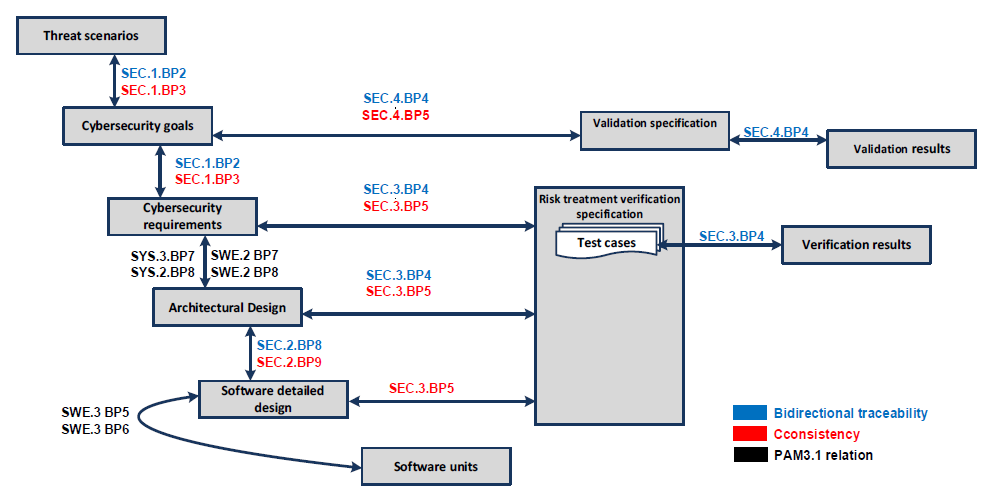
\includegraphics[width=150mm, keepaspectratio]{figures/02_ASPICE.png}
\caption{Az ASPICE javaslata kiberbiztonsági folyamatokra\cite{ASPICE}}
\label{fig:ASPICE}
\end{figure}

Szintén érdemes itt megjegyezni, hogy az általam javasolt metodológia egyfajta visszacsatolást (feedback) tenne lehetővé az \textit{Architectural design} és a \textit{Threat scenarios} lépések közt. De erről később bővebben lesz szó.

\subsection{UML és SysML}

\section{Felhasznált eszközök}
\subsection{Papyrus}
\subsection{Acceleo}
\subsection{Eclipse Modelling Framework}
\subsection{Xtend}
\subsection{Sirius}